\section{开发环境}\label{sec:DevelopmentEnvironment}

在本节(\cref{sec:DevelopmentEnvironment})中,笔者将对MinmusOS项目的开发环境进行介绍。

\subsection{基本概念}

\subsubsection{操作系统}

操作系统是一种控制计算机系统及其资源运行的软件。它有一个非常重要的通用特征:能够加载和执行用户程序,并为它们提供标准化的(与硬件无关的)输入/输出接口。

操作系统的主要功能可能包括:

\begin{enumerate}
    \item 管理内存和其他系统资源
    \item 实施安全和访问策略
    \item 调度和复用进程和线程
    \item 动态启动和关闭用户程序
    \item 提供基本的用户界面和应用程序编程接口
\end{enumerate}

并非所有的操作系统都提供所有这些功能。例如,单任务系统如MS-DOS不会调度进程,而嵌入式系统如eCOS可能没有用户界面,或者只能与一组静态的用户程序一起工作。

操作系统不是:

\begin{enumerate}
    \item 计算机硬件
    \item 特定的应用程序(如文字处理器、网页浏览器等)
    \item 一套实用程序(如在许多Unix派生系统中使用的GNU工具)
    \item 开发环境(尽管一些操作系统,如UCSD Pascal或Smalltalk-80,包含解释器和IDE)
    \item 图形用户界面(尽管许多现代操作系统将GUI作为操作系统的一部分)
\end{enumerate}

尽管大多数操作系统都会配备这些工具,但它们本身并不是操作系统的必要部分。一些操作系统,如Linux,可能以几种不同的打包形式分发,这些形式被称为发行版,它们可能拥有不同的应用程序和实用程序套件,并可能以不同的方式组织系统的某些方面。尽管如此,它们都是同一基本操作系统的版本,不应被视为不同类型的操作系统。

\subsubsection{内核}

内核是操作系统的核心部分,它负责处理所有基础级别的任务,尤其是与硬件直接交互的任务。内核的角色是桥接硬件和运行在计算机上的应用程序之间的通信。用户通常不会直接与内核交互,但它是系统运行的基础。

内核的主要职责包括:

\begin{enumerate}
    \item \textbf{中断处理}:内核响应由硬件产生的事件(称为中断)。例如,当按下键盘上的键时,内核的中断处理程序会获取按键编号,并将其转换成相应的字符存储在缓冲区中,供其他程序使用。
    \item \textbf{系统调用}:系统调用是用户级程序请求操作系统服务的方式。例如,打开文件、启动其他程序等。内核需要检查传入的参数是否有效,然后执行内部操作以完成请求。
    \item \textbf{资源管理}:内核管理计算机的资源,如CPU、内存和输入/输出设备。它负责资源的分配和回收,确保系统的高效运行。
    \item \textbf{进程调度}:内核负责进程和线程的调度。它决定哪个程序在何时使用CPU,以及如何在多个程序间公平地分配处理器时间。
    \item \textbf{抽象层}:内核通常定义一些基础的抽象概念,如文件、进程、套接字和目录等,这些都对应于它记住的关于上次操作的内部状态,使程序可以更高效地执行一系列操作。
\end{enumerate}

用户程序通常不直接发出系统调用(除了某些汇编程序),而是使用标准库来处理与内核交互所需的参数格式化和系统调用的生成。

总之,内核是操作系统最关键的组成部分,它提供了一个稳定和安全的环境,使得上层的应用程序能够不用关心硬件的复杂性而进行运行。

\subsubsection{Shell}

Shell是一个特殊的程序,通常集成在操作系统发行版中,为用户提供与计算机交互的界面。Shell的表现形式可能因系统而异(命令行、文件浏览器等),但其基本概念始终如一:

\begin{enumerate}
    \item \textbf{程序启动}:允许用户选择要启动的程序,并可选地给它提供特定于会话的参数。
    \item \textbf{文件操作}:允许对本地存储执行简单操作,如列出目录内容、在系统中移动和复制文件等。
\end{enumerate}

为了完成这些操作,Shell需要发出多个系统调用。Shell也可被其他程序用来启动程序。

现代的Shell还具有各种额外功能,包括:

\begin{enumerate}
    \item \textbf{自动补全}:通过按TAB键(或任何首选键),正在输入的单词将被自动补全为有效的Shell命令、文件、目录等。多次按自动完成键可以在其他补全可能性之间切换。
    \item \textbf{字符插入}:用户可以使用箭头键在输入的内容中移动。在句子中间键入新字符时,字符将被“插入”。
    \item \textbf{Shell历史记录}:通过使用上下箭头键,用户可以浏览之前的输入。
    \item \textbf{滚动}:当控制台的行数超过其高度时,将输出保存在缓冲区中,并允许用户在控制台中上下滚动。
    \item \textbf{脚本}:一些Shell具有自定义的脚本语言。脚本语言的例子包括Bash或DOS批处理。
\end{enumerate}

总之,Shell是操作系统中的一个核心组件,它通过友好的用户界面简化了用户与系统的交互,同时提供了执行复杂任务的强大命令行工具。

\subsubsection{GCC交叉编译器}

GCC交叉编译器(GCC Cross-Compiler)是一个特别定制的GCC(GNU Compiler Collection)编译器,它运行在一个平台(称为宿主平台,host),但生成的可执行文件却是为另一个平台(称为目标平台,target)设计的。这样的编译器使得开发者能在当前使用的操作系统(例如Windows或Linux)上开发针对完全不同的目标系统(如自制的操作系统或不同架构的嵌入式系统)的软件。

在实现操作系统内核时,使用GCC交叉编译器(GCC Cross-Compiler)是非常关键的,主要由于以下几个理由:

\begin{enumerate}
    \item \textbf{目标平台独立性}:开发操作系统时,正在创建的系统(目标系统)通常与当前使用的系统(宿主系统)不同。例如,在x86架构的Linux系统上开发针对ARM架构的嵌入式操作系统。GCC Cross-Compiler允许在宿主平台上编译出能在目标平台上运行的代码。
    \item \textbf{避免环境污染}:如果使用宿主系统的标准GCC编译器来编译内核代码,它可能会默认包含对宿主环境的依赖(如特定的系统调用、库函数或头文件),这可能导致编译出的内核在目标系统上无法正确运行。使用交叉编译器可以确保编译环境纯净,不会不小心引入宿主系统的元素。
    \item \textbf{正确处理系统调用和库函数}:交叉编译器能够提供适用于目标平台的系统调用和库函数接口,避免使用宿主平台的接口。这是因为操作系统内核需要对底层硬件进行直接管理,不能依赖宿主操作系统提供的抽象。
    \item \textbf{编译选项的正确设置}:交叉编译器允许开发者为目标平台精确配置编译器选项,如不使用标准库(使用\texttt{-nostdlib})、使用自由站立环境(使用\texttt{-ffreestanding})等,这些都是为了确保内核代码的独立性和正确执行。
    \item \textbf{简化开发过程}:一旦设置好交叉编译环境,后续的编译工作将变得简单和一致。开发者可以专注于内核的开发,而不需要担心编译环境可能引起的问题。
    \item \textbf{支持多平台}:通过不同的交叉编译器,可以在同一宿主系统上同时开发针对不同目标平台的操作系统版本。这种灵活性是使用宿主系统自带编译器所无法比拟的。
\end{enumerate}

因此,GCC Cross-Compiler在操作系统开发中是不可或缺的工具,它提供了从宿主平台到目标平台的无缝编译桥梁,确保了内核的正确编译和功能实现。这种方法不仅提高了开发效率,还保证了内核在目标环境中的稳定性和安全性。

\subsection{开发环境概述}

本项目的开发环境如下:

\begin{enumerate}
    \item 开发环境
          \begin{itemize}
              \item Windows 11 家庭中文版 23H2
              \item Ubuntu 22.04 LTS
              \item Windows Subsystem for Linux (WSL) 2.1.5.0
              \item QEMU 模拟机 v9.0.0
          \end{itemize}
    \item 开发软件
          \begin{itemize}
              \item Visual Studio Code
          \end{itemize}
    \item 开发语言
          \begin{itemize}
              \item C 语言
          \end{itemize}
\end{enumerate}

\subsubsection{Windows 11 家庭中文版 23H2}

使用Windows系统来开发操作系统内核,尽管可能不如Linux环境那样常见,但仍然有其独特的优势和便利性。以下是使用Windows系统开发操作系统内核的几个主要优势:

\begin{enumerate}
    \item \textbf{熟悉的开发环境}:对于习惯使用Windows的开发者来说,继续在这个环境下工作可以减少学习新工具和操作系统的时间,使他们能够更专注于开发工作本身。Windows的用户界面、文件系统管理、任务管理等都是开发者熟悉的。
    \item \textbf{强大的开发工具}:Windows支持多种强大的开发环境,如Visual Studio Code。这些IDE提供了先进的代码编辑、项目管理、版本控制和调试工具。
    \item \textbf{使用WSL提升开发效率}:通过集成了WSL(Windows Subsystem for Linux),Windows环境可以无缝地运行Linux工具和软件,结合了Linux的命令行工具和Windows的图形界面优势。这允许开发者在不离开Windows的情况下使用Linux环境,例如使用GCC、Make、GDB等工具进行内核开发。
    \item \textbf{文档和社区资源}:Windows拥有庞大的开发者社区和丰富的文档资源,对于解决开发中的问题和学习新技术都极为有用。
\end{enumerate}

总体而言,虽然Linux通常是内核开发的首选环境,但Windows提供的工具、支持和兼容性使其成为许多情况下一个可行且有效的选择,尤其是结合了WSL后,Windows在操作系统内核开发方面的适用性大大提高。

\subsubsection{Ubuntu 22.04 LTS 2.1.5.0}

使用Ubuntu作为开发环境,尤其是在开发操作系统内核这类底层项目时,有几个显著的优势:

\begin{enumerate}
    \item \textbf{稳定性和长期支持}:Ubuntu 22.04 LTS(Long Term Support,长期支持)版本提供了长达五年的安全更新和维护。这意味着开发者可以在一个稳定且长期受支持的平台上工作,无需担心频繁更换操作系统或缺乏安全更新。
    \item \textbf{与生产环境一致}:在Ubuntu上开发可以确保软件在生产环境中运行时表现得更加可靠和高效,因为开发和生产环境可以保持高度一致。
    \item \textbf{广泛的社区支持和资源}:Ubuntu拥有庞大的用户和开发者社区,这意味着大量的文档、论坛和支持资源可供查阅。这对于解决开发中遇到的问题非常有帮助。
    \item \textbf{开源工具和库的兼容性}:Ubuntu提供了丰富的开源开发工具和库。对于操作系统开发而言,这些工具(如GCC、Make、GDB)都是不可或缺的,而且通常在Linux系统上的兼容性和性能都非常好。
    \item \textbf{适合底层开发}:Linux系统提供了丰富的底层系统调用和接口,这对于内核开发是非常重要的。开发者可以直接与硬件和底层系统资源交互,更方便地实现和测试内核级功能。
    \item \textbf{环境一致性和隔离性}:使用容器和虚拟化技术(如Docker和QEMU),可以在Ubuntu上轻松创建和管理隔离的开发环境。这对于测试不同的配置和开发环境至关重要。
\end{enumerate}

总之,选择Ubuntu作为开发环境,可以为操作系统内核的开发提供一个稳定、高效、兼容性好的基础,同时也利于将来在类似环境中部署和运行。

\subsubsection{Windows Subsystem for Linux (WSL) 2.1.5.0}

使用 Windows Subsystem for Linux (WSL) 在开发操作系统内核时具有一系列优势,特别是对于习惯使用Windows环境的开发者来说。这些优势包括:

\begin{enumerate}
    \item \textbf{集成Windows和Linux环境}:WSL允许开发者在Windows系统上运行Linux环境,无需重启进入另一个操作系统或使用虚拟机。这意味着可以利用Windows的图形界面和生产力工具(如VSCode),同时执行Linux命令行工具和应用。
    \item \textbf{简化开发流程}:对于需要同时访问Windows和Linux工具的开发任务,WSL提供了极大的便利。开发者可以在相同的文件系统中访问项目文件,使用Windows编辑器编辑代码,然后在Linux环境中编译和测试,无需文件转移或复制。
    \item \textbf{资源占用更少}:与传统的虚拟机相比,WSL提供了更轻量级的解决方案。它直接在Windows内核上运行,减少了资源占用,启动和运行速度更快,对系统性能的影响也更小。
    \item \textbf{方便的环境管理}:WSL允许开发者安装多个Linux发行版,可以在不同的项目或任务之间切换不同的环境。例如,可以在一个发行版上进行开发工作,而在另一个发行版上进行测试。
    \item \textbf{直接访问硬件和系统调用}:WSL使用真实的Linux内核,这使得它在处理系统调用和操作硬件时表现得更接近传统Linux系统。这对于需要进行底层系统开发的项目尤其重要,因为它允许开发者在接近生产环境的条件下测试和开发。
    \item \textbf{持续集成和交叉编译支持}:使用WSL,开发者可以在同一机器上进行交叉编译,为不同的平台构建应用程序,包括Linux、Windows和其他操作系统。这种能力对于开发涉及多平台支持的内核或应用程序非常有用。
    \item \textbf{社区和官方支持}:Microsoft对WSL的持续更新和支持确保了其与现代硬件和软件技术的兼容性。此外,广泛的开发者社区也提供了大量的教程、工具和第三方应用支持,这对于解决开发中的问题非常有帮助。
\end{enumerate}

WSL是为那些想要在Windows系统上利用Linux开发工具的开发者提供了一种非常实用的解决方案,它结合了两个系统的优点,提高了开发效率和灵活性。

\subsubsection{QEMU 模拟机 v9.0.0}

QEMU是一个功能强大的开源机器模拟器和虚拟化解决方案,对于操作系统内核的开发尤为重要。以下是使用QEMU的一些主要优势:

\begin{enumerate}
    \item \textbf{多平台支持}:QEMU能够模拟多种处理器架构,包括x86、ARM、PowerPC、SPARC、和MIPS等。这意味着开发者可以在一个平台上开发和测试为其他平台设计的内核和应用程序,非常适合交叉平台开发。
    \item \textbf{环境隔离}:使用QEMU进行开发可以确保测试环境与主机操作系统隔离。这种隔离可以防止潜在的软件错误影响到主机系统,特别是在开发涉及底层硬件交互的系统软件时。
    \item \textbf{无需实际硬件}:QEMU允许开发者在没有物理目标硬件的情况下进行开发和测试。这不仅降低了成本,还可以在硬件到达前开始开发工作,加速开发周期。
    \item \textbf{调试支持}:QEMU与各种调试工具(如GDB)集成,可以进行详细的步进执行和调试。这对于操作系统内核开发尤为重要,因为它允许开发者在内核运行时进行观察和修改。
    \item \textbf{快照和即时状态保存}:QEMU支持保存和恢复虚拟机的状态(称为快照)。这使得开发者可以快速回滚到一个已知的良好状态,并从那里重新开始测试,极大地提高了测试的效率。
    \item \textbf{网络模拟}:QEMU还能模拟网络环境,允许开发者测试内核的网络功能,如协议栈和驱动程序,而无需实际的网络硬件。
    \item \textbf{性能和资源利用}:虽然QEMU为功能丰富性提供了强大的支持,但它在性能上的优化也非常有效。QEMU的用户模式模拟可以运行应用程序和驱动程序,而不必模拟整个操作系统,从而减少资源消耗。
    \item \textbf{版本更新和社区支持}:QEMU持续更新和改进,提供了最新的功能和改进,确保开发者可以利用最新的技术进行开发。同时,QEMU的广泛用户和开发者社区提供了丰富的文档、工具和支持。
\end{enumerate}

总体来说,QEMU提供了一个强大、灵活、成本效益高的平台,用于开发、测试和调试操作系统内核和其他系统级软件,特别是在多架构和虚拟化环境中。这使得它成为操作系统开发者的重要工具。

\subsubsection{Visual Studio Code}

使用 Visual Studio Code(VSCode)开发操作系统内核具有多方面的优势。VSCode是一款轻量级但功能强大的代码编辑器,它支持广泛的语言和工具,通过各种插件提供了强大的定制能力。以下是使用VSCode开发操作系统内核的主要优势:

\begin{enumerate}
    \item \textbf{高度可定制}:VSCode支持丰富的扩展库,这些插件为操作系统开发提供了必要的工具和功能,如WSL、对C语言的高级语法支持、代码格式化、以及链接脚本的编辑支持。
    \item \textbf{跨平台支持}:VSCode可在Windows、Linux和macOS上运行,这意味着开发环境可以跨平台保持一致性,便于团队协作和环境迁移。
    \item \textbf{集成终端和调试工具}:VSCode内置终端和强大的调试支持,可以直接在编辑器内部运行和调试代码。这对于内核开发尤其重要,因为它允许开发者快速测试和调试内核模块。
    \item \textbf{智能代码补全和语法高亮}:VSCode提供了智能的代码补全功能(IntelliSense)以及针对C/C++的语法高亮和错误提示,这极大地提高了编码效率和准确性。
    \item \textbf{代码格式化和风格一致性}:使用Clang-Format插件,可以自动格式化代码以符合预设的编码风格,确保代码的整洁和一致性。这对于团队开发尤其重要,能够保持代码风格统一。
    \item \textbf{轻量级和高性能}:VSCode本身是轻量级的,不像一些重型集成开发环境(IDE)那样消耗大量系统资源。它的启动和运行速度快,对系统的干扰小。
    \item \textbf{广泛的社区支持和插件生态}:VSCode拥有活跃的开发者社区和庞大的插件生态系统,这意味着它经常更新和改进,开发者可以轻松找到解决问题的资源和新的工具。
    \item \textbf{版本控制集成}:VSCode有良好的版本控制系统支持,尤其是对Git的集成,这使得管理复杂的开发项目变得更加容易。
\end{enumerate}

总之,使用VSCode开发操作系统内核可以提供一个灵活、高效、并且功能丰富的开发环境,非常适合现代操作系统开发的需求。

\subsubsection{C 语言}

使用C语言开发操作系统内核具有许多显著的优势,这也是为什么C语言在系统编程领域中非常流行和重要。以下是使用C语言开发操作系统内核的几个主要优势:

\begin{enumerate}
    \item \textbf{接近硬件的操作能力}:C语言提供了丰富的底层操作能力,允许开发者直接管理硬件资源,如内存地址和硬件设备。这种能力对于操作系统内核的开发至关重要,因为内核需要直接与硬件交互,管理内存、处理器、I/O设备等。
    \item \textbf{性能效率}:C语言生成的代码在执行效率上非常高,这是因为它产生接近汇编语言的机器代码,减少了运行时的开销。在操作系统内核中,每一点性能都非常宝贵,因为它直接影响到整个系统的响应速度和效率。
    \item \textbf{控制和灵活性}:C语言提供了极大的控制能力,例如通过指针操作内存。这种精细的控制能力允许开发者优化数据结构和算法,精确管理资源的使用,这在内核开发中是非常重要的。
    \item \textbf{可移植性}:虽然C语言允许底层访问,但其编写的程序在不同的平台(具有相应的编译器支持)上具有良好的可移植性。操作系统内核可以在一种硬件平台上开发和测试,然后相对容易地迁移到其他硬件平台。
    \item \textbf{广泛的支持和社区}:C语言是一种历史悠久且广泛使用的语言,有大量的文献、工具和社区支持。对于开发操作系统内核这样的复杂项目,强大的社区支持可以提供丰富的资源。
    \item \textbf{成熟的工具链}:C语言拥有成熟的编译器和调试工具,如GCC、Clang、GDB等。这些工具在操作系统开发中非常重要,因为它们可以帮助开发者发现和修复底层代码的问题。
    \item \textbf{标准库和第三方库}:尽管在内核开发中可能不会频繁使用标准库,但C语言的标准库提供了基础的数据操作和算法,而且有许多第三方库可以用于测试和模拟内核行为。
    \item \textbf{历史和遗产}:许多现代操作系统的内核,如Unix/Linux的内核,最初是用C语言编写的。使用C语言继续开发和维护这些内核有助于保持代码的一致性和理解性。
\end{enumerate}

总结来说,C语言在操作系统内核开发中之所以占据主导地位,是因为它提供了与硬件紧密交互的能力、高性能的代码执行、以及对底层系统资源的精细控制。这些特点使得C语言非常适合需要直接硬件控制和高性能要求的操作系统内核开发。

\subsection{开发环境搭建}

\subsubsection{配置Visual Studio Code及其扩展}

Visual Studio Code(VSCode)是一款由微软开发的免费、开源的代码编辑器。它支持Windows、macOS和Linux操作系统。VSCode能够支持多种编程语言,并且通过扩展库可以支持更多功能。

下面是配置Visual Studio Code及其扩展的步骤:

\begin{enumerate}
    \item 在VSCode官网(\url{https://code.visualstudio.com})下载并安装VSCode(\cref{fig:VSCodeWebsite})
          \begin{figure}[htbp]
              \centering
              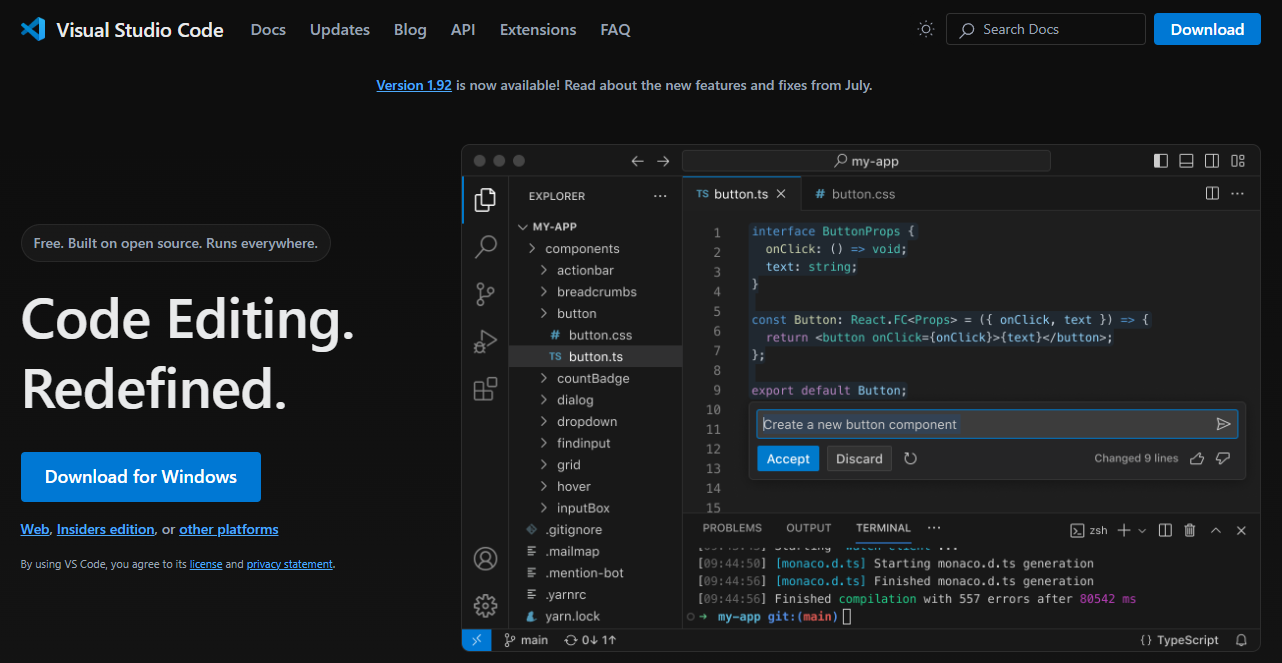
\includegraphics[width=0.8\textwidth]{figures/VSCodeWebsite.png}
              \caption{Visual Studio Code官网}
              \label{fig:VSCodeWebsite}
          \end{figure}
    \item 在VSCode中向本地安装扩展:Chinese (Simplified) (简体中文) Language Pack for Visual Studio Code,以支持简体中文语言(\cref{fig:VSCodeLocalExtensions})
    \item 在VSCode中向本地安装扩展:LinkerScript,以支持LinkerScript语言(\cref{fig:VSCodeLocalExtensions})
    \item 在VSCode中向本地安装扩展:WSL,以允许用户在Windows中使用Linux环境(\cref{fig:VSCodeLocalExtensions})
          \begin{figure}[htbp]
              \centering
              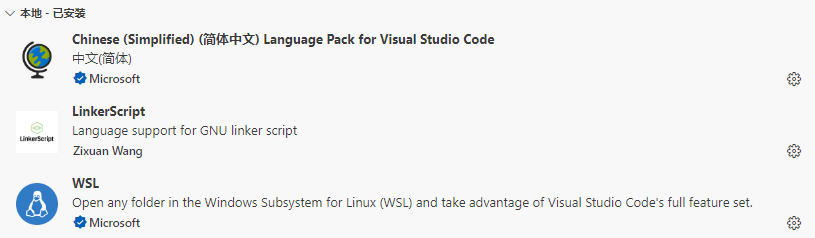
\includegraphics[width=0.8\textwidth]{figures/VSCodeLocalExtensions.png}
              \caption{VSCode本地扩展}
              \label{fig:VSCodeLocalExtensions}
          \end{figure}
\end{enumerate}

\subsubsection{配置WSL: Ubuntu 22.04 LTS}

WSL是一个在Windows操作系统上运行Linux环境的兼容层,允许用户直接在Windows中安装和使用Linux环境。Ubuntu 22.04 LTS可以为操作系统内核的开发提供一个稳定、高效、兼容性好的基础,同时也利于将来在类似环境中部署和运行。

下面是配置WSL: Ubuntu 22.04 LTS的步骤:

\begin{enumerate}
    \item 在“控制面板”>“程序”>“程序和功能”>“启用或关闭Windows功能”中,确定“适用于Linux的Windows子系统”已被选中。
    \item 在“Windows任务管理器”>“性能”>“CPU”选项卡中,确定“虚拟化”已启用(\cref{fig:WindowsTaskManager})。
          \begin{figure}[htbp]
              \centering
              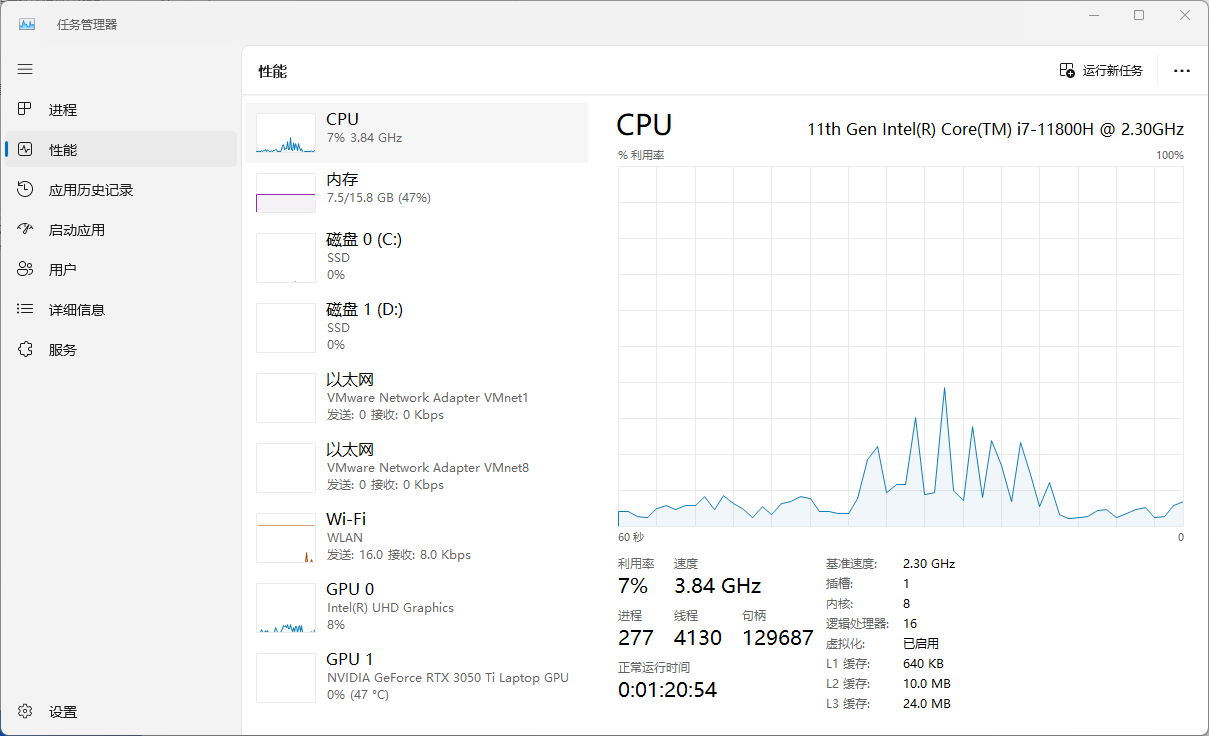
\includegraphics[width=0.8\textwidth]{figures/WindowsTaskManager.png}
              \caption{Windows任务管理器}
              \label{fig:WindowsTaskManager}
          \end{figure}
    \item 启动Windows PowerShell,执行\cref{lst:ConfigureUbuntu},以配置Ubuntu 22.04 LTS操作系统。这段代码的作用分别是:
          \begin{itemize}
              \item \texttt{wsl --version}:显示当前WSL的版本信息
              \item \texttt{wsl --install Ubuntu-22.04}:安装Ubuntu 22.04 LTS版本到WSL
              \item \texttt{wsl --list}:列出所有已安装的Linux发行版
          \end{itemize}
          代码执行结果如\cref{fig:ConfigureUbuntu}。
          \begin{listing}[htbp]
              \begin{minted}{bash}
wsl --version
wsl --install Ubuntu-22.04
wsl --list
          \end{minted}
              \caption{配置WSL: Ubuntu 22.04 LTS}\label{lst:ConfigureUbuntu}
          \end{listing}
          \begin{figure}[htbp]
              \centering
              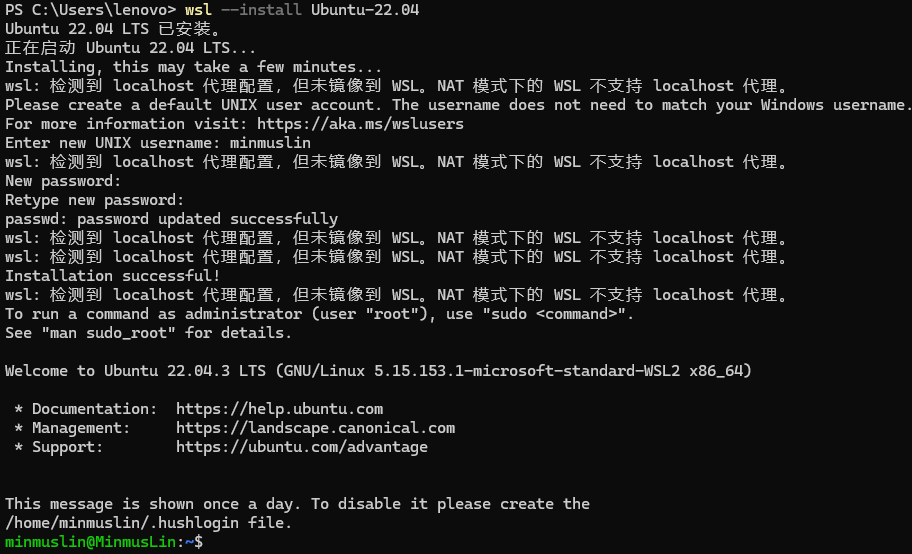
\includegraphics[width=0.8\textwidth]{figures/ConfigureUbuntu.png}
              \caption{配置WSL: Ubuntu 22.04 LTS}
              \label{fig:ConfigureUbuntu}
          \end{figure}
    \item 启动VSCode,选择窗口左下角“打开远程窗口”,选择“使用发行版连接到WSL...”,继续选择“Ubuntu-22.04默认发行版”,窗口左下角提示“正在打开远程...”并正在启动Linux子系统,当窗口左下角提示“WSL: Ubuntu-22.04”时说明已连接到WSL(\cref{fig:ConnectedToWSL})。
          \begin{figure}[htbp]
              \centering
              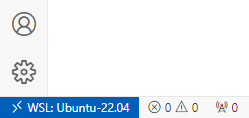
\includegraphics[]{figures/ConnectedToWSL.png}
              \caption{已连接到WSL}
              \label{fig:ConnectedToWSL}
          \end{figure}
\end{enumerate}

\subsubsection{配置C语言开发环境}

C语言在操作系统内核的开发中起着关键作用,因为它提供了接近硬件的低级访问能力,同时保持足够的抽象,以便于管理和编写复杂的系统级代码。

下面是配置C语言开发环境的步骤:

\begin{enumerate}
    \item 在VSCode中通过WSL连接到Ubuntu 22.04 LTS(\cref{fig:ConnectedToWSL})
    \item 在VSCode中向WSL: Ubuntu-22.04安装扩展:C/C++,以支持C语言(\cref{fig:VSCodeWSLExtensions})
    \item 在VSCode中向WSL: Ubuntu-22.04安装扩展:Clang-Format,以支持C语言代码格式化(\cref{fig:VSCodeWSLExtensions})
          \begin{figure}[htbp]
              \centering
              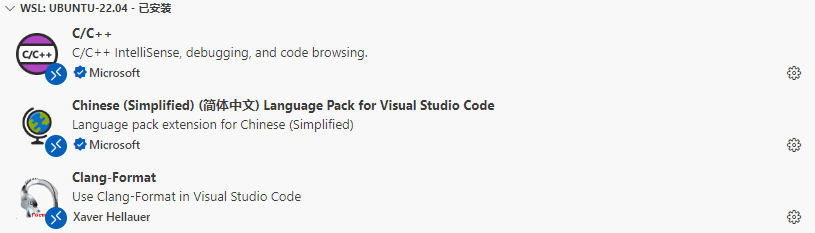
\includegraphics[width=0.8\textwidth]{figures/VSCodeWSLExtensions.png}
              \caption{VSCode WSL: Ubuntu-22.04 扩展}
              \label{fig:VSCodeWSLExtensions}
          \end{figure}
\end{enumerate}

\subsubsection{配置\texttt{i686-elf-gcc}交叉编译环境}

\texttt{i686-elf-gcc}是一个特定类型的GCC交叉编译器。它用于编译生成可在i686架构的无操作系统环境(bare-metal)中运行的代码。这里,“i686”指的是Intel和兼容处理器的32位指令集架构,通常用于较旧的Intel Pentium和兼容CPU。而“elf”表示生成的目标文件格式是ELF(Executable and Linkable Format),这是在多种Unix-like系统中使用的一种常见文件格式。

下面是配置\texttt{i686-elf-gcc}交叉编译环境的步骤:

\begin{enumerate}
    \item 在VSCode中通过WSL连接到Ubuntu 22.04 LTS(\cref{fig:ConnectedToWSL}),并启动终端,在终端中执行\cref{lst:InstallDependencies}以安装依赖。这段代码的作用分别是:
          \begin{itemize}
              \item \texttt{sudo apt update}:更新本地软件包索引,在安装新软件包前确保可以访问到最新的软件包版本
              \item \texttt{sudo apt install -y}:安装一系列软件包,\texttt{-y}参数表示自动同意安装过程中的询问
                    \begin{itemize}
                        \item \texttt{build-essential}:这个包包含了编译软件所必需的一些基本工具(如gcc编译器、g++、make等),这是编译大多数软件(包括交叉编译器)所必需的
                        \item \texttt{bison}:Bison是一个语法分析器生成器,它通常用于复杂的语言处理软件或编程语言的编译器的开发
                        \item \texttt{flex}:Flex是一个快速的词法分析器生成器,用于生成程序的词法分析部分,它与Bison配合使用生成编译器的前端
                        \item \texttt{libgmp3-dev}:GMP(GNU多精度库)是一种允许高精度算术的库,GCC编译过程中用来处理数学计算
                        \item \texttt{libmpc-dev}:MPC是一个复数算术的C语言库,GCC用它来进行复杂的算术运算,尤其是在编译过程中处理浮点运算
                        \item \texttt{libmpfr-dev}:MPFR提供了一种用于多精度浮点数计算的库,它为GCC的浮点运算提供了支持
                        \item \texttt{texinfo}:Texinfo是一个官方的GNU文档系统,用于编写可转换成多种格式的文档和手册
                        \item \texttt{grub-common}、\texttt{grub-pc-bin}:这些包与GRUB相关,一个是GRUB的通用文件,另一个是GRUB的二进制文件。GRUB是一个多操作系统引导加载程序,用于编译操作系统内核并创建可启动的ISO映像
                        \item \texttt{xorriso}:用于创建、修改和抽取ISO文件。在创建可启动的操作系统光盘映像时需要这个工具
                        \item \texttt{clang-format}:用于自动格式化C语言代码,保持代码风格的一致性
                    \end{itemize}
          \end{itemize}
          \begin{listing}[htbp]
              \begin{minted}{bash}
sudo apt update && \
sudo apt install -y \
    build-essential \
    bison \
    flex \
    libgmp3-dev \
    libmpc-dev \
    libmpfr-dev \
    texinfo \
    grub-common \
    grub-pc-bin \
    xorriso \
    clang-format
          \end{minted}
              \caption{安装依赖}\label{lst:InstallDependencies}
          \end{listing}
    \item 为简化构建\texttt{i686-elf-gcc}交叉编译器的流程,\texttt{Appendix}附录文件夹中提供了Shell脚本文件\texttt{build\_i686\_elf\_gcc.sh},将这份用于构建\texttt{i686-elf-gcc}交叉编译器的Shell脚本文件复制到\texttt{\textbackslash\textbackslash wsl.localhost\textbackslash Ubuntu-22.04\textbackslash home\textbackslash <Username>}路径下,其中\texttt{<Username>}为Ubuntu操作系统的用户名,Shell脚本文件\texttt{build\_i686\_elf\_gcc.sh}的作用如下:
          \begin{itemize}
              \item 初始化变量(\cref{lst:InitializeVariables})
                    \begin{itemize}
                        \item 这部分定义了必要的变量,如Binutils和GCC的版本号和下载链接,Binutils版本为2.37,GCC版本为11.2.0
                        \item 设置了安装路径\texttt{PREFIX}和目标平台\texttt{TARGET}
                        \item 将交叉编译器的\texttt{bin}目录添加到环境变量\texttt{PATH}中
                    \end{itemize}
                    \begin{listing}[htbp]
                        \begin{minted}{bash}
#!/usr/bin/bash

BINUTIL_VERSION=2.37
BINUTIL_URL="https://mirrors.aliyun.com/gnu/binutils/binutils-2.37.tar.xz?" \
            "spm=a2c6h.25603864.0.0.5f4539e11JPeX4"

GCC_VERSION=11.2.0
GCC_URL="https://mirrors.aliyun.com/gnu/gcc/gcc-11.2.0/gcc-11.2.0.tar.xz?" \
        "spm=a2c6h.25603864.0.0.6c5d9698I99N4Y"

GCC_SRC="gcc-${GCC_VERSION}"
BINUTIL_SRC="binutils-${BINUTIL_VERSION}"

export PREFIX="$HOME/cross-compiler"
export TARGET=i686-elf
export PATH="$PREFIX/bin:$PATH"
                    \end{minted}
                        \caption{\texttt{build\_i686\_elf\_gcc.sh}:初始化变量}\label{lst:InitializeVariables}
                    \end{listing}
              \item 创建目录(\cref{lst:CreateDirectories})
                    \begin{itemize}
                        \item 这些命令创建了用于存放编译器和构建文件的目录
                    \end{itemize}
                    \begin{listing}[htbp]
                        \begin{minted}{bash}
mkdir -p "${PREFIX}"
mkdir -p "${HOME}/toolchain/binutils-build"
mkdir -p "${HOME}/toolchain/gcc-build"
                    \end{minted}
                        \caption{\texttt{build\_i686\_elf\_gcc.sh}:创建目录}\label{lst:CreateDirectories}
                    \end{listing}
              \item 下载和解压Binutils和GCC源码(\cref{lst:DownloadAndExtractSourceCode})
                    \begin{itemize}
                        \item 检查是否已下载并解压了GCC和Binutils的源代码,如果没有则下载并解压
                        \item 使用\texttt{wget}命令下载,并使用\texttt{tar}解压缩
                    \end{itemize}
                    \begin{listing}[htbp]
                        \begin{minted}{bash}
cd "${HOME}/toolchain"

if [ ! -d "${HOME}/toolchain/${GCC_SRC}" ]
then
    (wget -O "${GCC_SRC}.tar" ${GCC_URL} \
        && tar -xf "${GCC_SRC}.tar") || exit
    rm -f "${GCC_SRC}.tar"
else
    echo "Skip downloading gcc"
fi

if [ ! -d "${HOME}/toolchain/${BINUTIL_SRC}" ]
then
    (wget -O "${BINUTIL_SRC}.tar" ${BINUTIL_URL} \
        && tar -xf "${BINUTIL_SRC}.tar") || exit
    rm -f "${BINUTIL_SRC}.tar"
else
    echo "Skip downloading binutils"
fi
                    \end{minted}
                        \caption{\texttt{build\_i686\_elf\_gcc.sh}:下载和解压Binutils和GCC源码}\label{lst:DownloadAndExtractSourceCode}
                    \end{listing}
              \item 构建Binutils 2.37(\cref{lst:BuildBinutils})
                    \begin{itemize}
                        \item 进入Binutils构建目录
                        \item 配置构建选项,指定目标架构、安装路径,禁用本地化和警告
                        \item 使用\texttt{make}构建并安装
                    \end{itemize}
                    \begin{listing}[htbp]
                        \begin{minted}{bash}
echo "Building Binutils 2.37 ..."

cd "${HOME}/toolchain/binutils-build"

("${HOME}/toolchain/${BINUTIL_SRC}/configure" \
    --target=$TARGET \
    --prefix="$PREFIX" \
    --with-sysroot \
    --disable-nls \
    --disable-werror) || exit

(make && make install) || exit
                    \end{minted}
                        \caption{\texttt{build\_i686\_elf\_gcc.sh}:构建Binutils 2.37}\label{lst:BuildBinutils}
                    \end{listing}
              \item 构建GCC 11.2.0(\cref{lst:BuildGCC})
                    \begin{itemize}
                        \item 进入GCC构建目录
                        \item 检查\texttt{as}汇编器是否在路径中
                        \item 配置GCC构建选项,包括支持的语言和其他编译选项
                        \item 分步骤构建GCC和libgcc,然后安装
                    \end{itemize}
                    \begin{listing}[htbp]
                        \begin{minted}{bash}
echo "Building GCC 11.2.0 ..."

cd "${HOME}/toolchain/gcc-build"

which -- "$TARGET-as" || echo "$TARGET-as is not in the PATH"

("${HOME}/toolchain/${GCC_SRC}/configure" \
    --target=$TARGET \
    --prefix="$PREFIX" \
    --disable-nls \
    --enable-languages=c,c++ \
    --without-headers) || exit

(make all-gcc && \
    make all-target-libgcc && \
    make install-gcc && \
    make install-target-libgcc) || exit

echo "Done"
                    \end{minted}
                        \caption{\texttt{build\_i686\_elf\_gcc.sh}:构建GCC 11.2.0}\label{lst:BuildGCC}
                    \end{listing}
          \end{itemize}
    \item 在终端中执行\cref{lst:ConfigureCrossCompiler}以配置\texttt{i686-elf-gcc}交叉编译环境。这段代码的作用分别是:
          \begin{itemize}
              \item \texttt{ls}:列出当前目录中的所有文件和文件夹,确认Shell脚本文件\texttt{build\_i686\_elf\_gcc.sh}存在于目录中
              \item \texttt{chmod u+x build\_i686\_elf\_gcc.sh}:修改文件\texttt{build\_i686\_elf\_gcc.sh}的权限,使得文件的所有者(user,标记为\texttt{u})具有执行(execute,标记为\texttt{x})该文件的权限
              \item \texttt{./build\_i686\_elf\_gcc.sh}:执行Shell脚本文件\texttt{build\_i686\_elf\_gcc.sh}
          \end{itemize}
          \begin{listing}[htbp]
              \begin{minted}{bash}
ls
chmod u+x build_i686_elf_gcc.sh
./build_i686_elf_gcc.sh
          \end{minted}
              \caption{配置\texttt{i686-elf-gcc}交叉编译环境}\label{lst:ConfigureCrossCompiler}
          \end{listing}
    \item 为单个用户添加环境变量
          \begin{itemize}
              \item 在终端中执行\cref{lst:EditBashrc},打开当前用户\texttt{home}目录下的\texttt{.bashrc}文件进行编辑
                    \begin{listing}[htbp]
                        \begin{minted}{bash}
nano ~/.bashrc
                    \end{minted}
                        \caption{编辑\texttt{.bashrc}文件}\label{lst:EditBashrc}
                    \end{listing}
              \item 在\texttt{.bashrc}文件的底部添加\cref{lst:ModifyBashrc},这会将路径添加到现有的\texttt{PATH}环境变量前面,确保此目录中的程序可以被优先找到
                    \begin{listing}[htbp]
                        \begin{minted}{bash}
export PATH="$HOME/cross-compiler/bin:$PATH"
                    \end{minted}
                        \caption{修改\texttt{.bashrc}文件}\label{lst:ModifyBashrc}
                    \end{listing}
              \item 保存并关闭文件。如果使用nano编辑器,可以按Ctrl+X,然后按Y键保存更改,再按Enter键退出
              \item 为了使\texttt{.bashrc}文件的更改立即生效,在终端中执行\cref{lst:SourceBashrc},重新加载文件以应用更改
                    \begin{listing}[htbp]
                        \begin{minted}{bash}
source ~/.bashrc
                    \end{minted}
                        \caption{加载\texttt{.bashrc}文件}\label{lst:SourceBashrc}
                    \end{listing}
          \end{itemize}
    \item 在终端中执行\cref{lst:VerifyCrossCompiler}验证\texttt{i686-elf-gcc}交叉编译环境是否配置成功,这段代码的作用分别是:
          \begin{itemize}
              \item \texttt{i686-elf-gcc --version}:显示\texttt{i686-elf-gcc}编译器的版本信息
              \item \texttt{i686-elf-gcc -dumpmachine}:输出编译器的目标机器的三元组描述(target triplet),即编译器为其生成代码的平台,这指明编译器生成的代码是为了运行在i686架构的裸机环境(无操作系统)中
          \end{itemize}
          代码执行结果分别为\texttt{i686-elf-gcc (GCC) 11.2.0}和\texttt{i686-elf}则说明\texttt{i686-elf-gcc}交叉编译环境配置成功
          \begin{listing}[htbp]
              \begin{minted}{bash}
i686-elf-gcc --version
i686-elf-gcc -dumpmachine
          \end{minted}
              \caption{验证\texttt{i686-elf-gcc}交叉编译环境}\label{lst:VerifyCrossCompiler}
          \end{listing}
\end{enumerate}

\subsubsection{配置QEMU模拟机v9.0.0}

QEMU是一种功能强大的虚拟机模拟器,它可以用于开发操作系统内核,允许开发者在隔离和控制的环境中测试和调试新的操作系统代码,而无需在真实硬件上运行。

下面是配置QEMU模拟机v9.0.0的步骤:

\begin{enumerate}
    \item 在QEMU官网(\url{https://www.qemu.org})下载并安装QEMU模拟机v9.0.0(\cref{fig:QEMUWebsite})
          \begin{figure}[htbp]
              \centering
              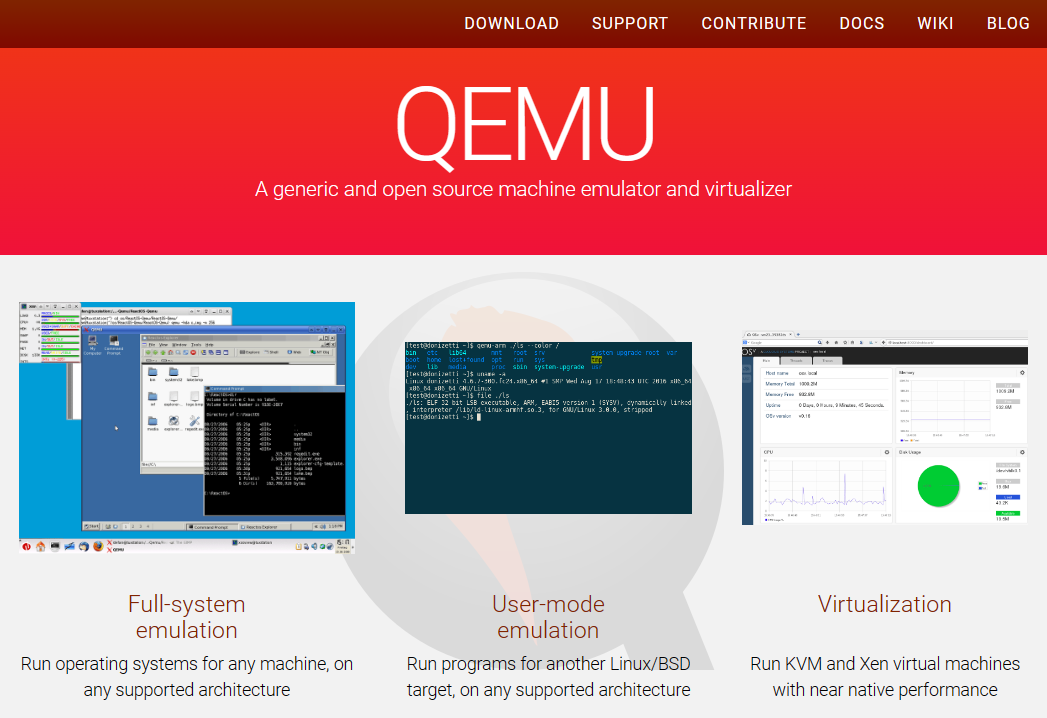
\includegraphics[width=0.8\textwidth]{figures/QEMUWebsite.png}
              \caption{Visual Studio Code官网}
              \label{fig:QEMUWebsite}
          \end{figure}
    \item 将QEMU的安装路径添加到系统环境变量,以便在任何命令行界面中直接调用QEMU,而不需要每次都输入完整的路径
          \begin{itemize}
              \item 找到QEMU的安装路径
              \item 打开系统环境变量编辑界面:“设置”>“系统”>“系统信息”>“高级系统设置”>“环境变量”
              \item 编辑系统环境变量:在“环境变量”窗口中,找到“系统变量”区域,然后滚动找到变量\texttt{Path},并选择它,点击“编辑”按钮,之后点击“新建”按钮,在新的行输入QEMU的安装路径,确认无误后,点击“确定”保存更改
              \item 应用更改:在所有环境变量窗口中点击“确定”以应用更改并关闭窗口,重启命令行界面(如命令提示符或PowerShell),新的环境变量设置将立即生效
          \end{itemize}
    \item 在Windows命令提示符中执行\cref{lst:VerifyQEMU}验证QEMU模拟机v9.0.0是否配置成功,正确显示版本信息则说明QEMU模拟机v9.0.0配置成功
          \begin{listing}[htbp]
              \begin{minted}{bash}
qemu-system-i386 --version
          \end{minted}
              \caption{验证QEMU模拟机v9.0.0}\label{lst:VerifyQEMU}
          \end{listing}
\end{enumerate}

\subsection{运行MinmusOS项目}